\chapter{Introduction}

\dictum[Теодо́сій Григо́рович Добжа́нський (Theodosius
Dobzhansky)\footnotemark]{Nothing in biology makes sense}
\footnotetext{\citet{Dobzhansky:1973}}

\section{The central dogma}

At the core of every living being is its genetic inheritance. The genetic
inheritance is what is being passed down from parents to their offspring, and
contains a blueprint detailing how to construct a new individual in a process
called \define{embryogenesis}. This genetic inheritance is physically present in
the form of \dna in every living cell.\footnote{And to some extent in non-living
particles called \define{viruses}.}

If the \dna is a library containing a blueprint of the cell’s instructions, then
there is need also for librarians, and for workers who enact the instructions
found in the blueprint and conveyed by the librarians. These find their
counterparts in living cells in the form of \mrna and \define{proteins}. The
process by which genetic information is stored in the \dna, conveyed by
\mrna[s], and enacted by proteins is formalised in the \emph{central dogma of
molecular biology}.

\begin{figure}[h!]
    \centering
    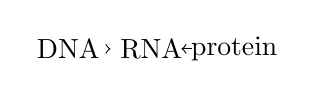
\begin{tikzpicture}
        [every node={circle, draw, inner sep=1em}, node distance=3em]
        \node (dna) {DNA};
        \node (rna) [right of=dna] {RNA};
        \node (protein) [right of=rna] {protein};
        \draw [->] (dna) -- (rna);
        \draw [->] (rna) -- (protein);
    \end{tikzpicture}
    \figcap{dogma}{The central dogma of molecular biology.}{}
\end{figure}

This very high-level view needs to be complemented by a more mechanistic
description in order to make sense. All three roles in the central dogma are
fulfilled by different molecules. \dna consists of a long chain of
\define{nucleotides}. The chemical nature of nucleotides means that these will
easily polymerase into long, relatively stable chains. \dna is made up of four
different types of nucleotides: adenine (\nA), cytosine (\nC), guanine (\nG) and
thymine (\nT). Thus, \dna can be thought of as a long string of four different
letters, and that is indeed how it is often represented. Text is read from left
to right in Western cultures. \dna is read from \fivep to
\threep.\footnote{Referring to the number of the phosphate atom in each
nucleotide, which is exposed at either end of the chain.}

\dna is present in the cell in the form of double-stranded helices: each \dna
molecule consists of two paired chains, wound rightly around each other, with
the bases on each chain pairing up such that every \nA on one chain is paired
with a \nT on the other, and each \nC is paired with a \nG. This striking
symmetry is known as Watson–Crick base pairing, after its discoverers
\citep{Watson:1953}. Thus, \dna is made up of two complementary strands,
redundantly holding the genetic information. This redundancy is used in \dna
copying (which occurs at every cell division, and is the mechanism by which
genetic information is passed from one cell to its offspring) to synthesise two
newly formed \dna molecules, of which each contains one strand of the parent
\dna molecule (\define{semiconservative replication}).

\todo[inline]{\begin{enumerate}[noitemsep,nolistsep,leftmargin=*]
    \item Molecular structure of DNA (bases, 5'--3', phosphoribose)
    \item DNA copying (strands, complementarity)
    \item Central dogma
    \item Template, coding strand, mRNA, proteins, genetic code
    \item Different polymerases, ncRNA
    \item DNA sequence as string
    \item Molecular and functional structure description of pol2 and pol3
    \item Structure of a tRNA gene (internal promoters etc.)
    \item tRNA modification, (re)loading and degradation: life-cycle has impact
        on abundance, and thus on translation efficiency. We completely ignore
        this; but why can we do this?
    \item Genetic code, anticodon isoacceptors, tRNA genes, wobble base pairing
    \item tAI, codon usage, codon usage bias, anticodon abundance bias
    \item Tiny bit about mouse embryonology
    \item Prior research/literature review of tRNA and codon usage, also outside
        mammals!
\end{enumerate}}

\todo{Take intro from paper}

\section{The genetic code}

The \mrna formed during transcription is subsequently \define{translated} into a
protein. This requires the conversion of the information represented on the
\mrna using \num{4} nucleotides  into a different code, that of the protein.
Proteins are polypeptides: chains of amino acids. Each amino acid is a small
molecule with unique properties, which, together, shape the function of the
final protein. Individual amino acids are strung together in a chemical reaction
that links a carboxyl group covalently with an amino group on the next amino
acid to form a \define{peptide bond} (\ce{-COOH + -NH2 -> -CO-NH\bond{-} +
H2O}) \citep{Alberts:2002}.

There are \num{20} different amino acids that are coded for by just \num{4}
different nucleotides. To enable this, several nucleotides must be combined to
form a larger unit coding for an amino acid. In the universal genetic code,
shared by all known species, this is accomplished by grouping three consecutive
nucleotides together to form \define{codons} along the \mrna. This results in
\(4^3 = 64\) possible codons, vastly more than there are amino acids. As a
consequence, the genetic code is \define{degenerate}: several codons code for
the same amino acid. In addition to encoding the amino acid methionine, one
codon, \codon{AUG} marks the site of translation initiation; three codons do not
encode any amino acid, and instead signal the stop of translation (\codon{UAA},
\codon{UAG}, \codon{UGA}).

The translation of \mrna into proteins is assisted by a special apparatus called
the \define{ribosome}. Ribosomes are large complexes of proteins and \rrna,
forming two subunits. In eukaryotes, these subunits are the 40S and 60S subunit,
respectively. During translation initiation, the two subunits assemble on the
\mrna molecule at the site of the translation initiation codon. The ribosome
then pulls the \mrna through a channel in its structure and progressively
translates the \mrna into amino acids, which are chained together to form a
nascent polypeptide chain.

Individual codons are translated into their corresponding amino acid by aid of
specific adapter molecules carrying a specific amino acid, and which recognise
the matching codon. This codon recognition is possible because the adapter
molecules are themselves \abbr{rna}s, and the codon is matched via complementary
base pairing of a part of the \rna sequence termed the \define{anticodon}. These
adapter molecules are called \define{\trna}.

\Cref{tab:genetic-code} contains a tabular representation of the genetic code,
which is nearly universal across all three domains of life. To avoid confusion,
codons in this thesis will always be typeset like this:
\fivep--\codon{CAU}--\threep; anticodons will always be typeset like this:
\threep--\anticodon{ATG}--\fivep (directions given here only, not in the
remainder of the text).

\begin{table}
    \centering
    \def\s{\footnotesize stop}
    \def\h#1#2{\multicolumn{1}{#1}{\textsc{\lowercase{#2}}}}
    \begin{tabu} to \textwidth {@{}
            >{\collectcell\codon}l<{\endcollectcell}
            >{\collectcell\anticodon}l<{\endcollectcell}
            l @{\qquad}
            >{\collectcell\codon}l<{\endcollectcell}
            >{\collectcell\anticodon}l<{\endcollectcell}
            l @{\qquad}
            >{\collectcell\codon}l<{\endcollectcell}
            >{\collectcell\anticodon}l<{\endcollectcell}
            l @{\qquad}
            >{\collectcell\codon}l<{\endcollectcell}
            >{\collectcell\anticodon}l<{\endcollectcell}
            l @{}}
        \toprule
        % Nasty, hand-coded length values.
        \noalign{\vskip-4pt}
        \h{@{}l}{C} & \h{l}{A} & \h{l}{AA} &
        \h{@{}l}{C} & \h{l}{A} & \h{l}{AA} &
        \h{@{}l}{C} & \h{l}{A} & \h{l}{AA} &
        \h{@{}l}{C} & \h{l}{A} & \h{l@{}}{AA} \\[-2pt]
        \midrule
        UUU & AAA & Phe & UCU & AGA & Ser & UAU & ATA & Tyr & UGU & ACA & Cys \\
        UUC & GAA & Phe & UCC & GGA & Ser & UAC & GTA & Tyr & UGC & GCA & Cys \\
        UUA & TAA & Leu & UCA & TGA & Ser & UAA & TTA & \s  & UGA & TCA & \s \\
        UUG & CAA & Leu & UCG & CGA & Ser & UAG & CTA & \s  & UGG & CCA & Trp \\
        \addlinespace
        CUU & AAG & Leu & CCU & AGG & Pro & CAU & ATG & His & CGU & ACG & Arg \\
        CUC & GAG & Leu & CCC & GGG & Pro & CAC & GTG & His & CGC & GCG & Arg \\
        CUA & TAG & Leu & CCA & TGG & Pro & CAA & TTG & Gln & CGA & TCG & Arg \\
        CUG & CAG & Leu & CCG & CGG & Pro & CAG & CTG & Gln & CGG & CCG & Arg \\
        \addlinespace
        AUU & AAT & Ile & ACU & AGT & Thr & AAU & ATT & Asn & AGU & ACT & Ser \\
        AUC & GAT & Ile & ACC & GGT & Thr & AAC & GTT & Asn & AGC & GCT & Ser \\
        AUA & TAT & Ile & ACA & TGT & Thr & AAA & TTT & Lys & AGA & TCT & Arg \\
        AUG & CAT & Met & ACG & CGT & Thr & AAG & CTT & Lys & AGG & CCT & Arg \\
        \addlinespace
        GUU & AAC & Val & GCU & AGC & Ala & GAU & ATC & Asp & GGU & ACC & Gly \\
        GUC & GAC & Val & GCC & GGC & Ala & GAC & GTC & Asp & GGC & GCC & Gly \\
        GUA & TAC & Val & GCA & TGC & Ala & GAA & TTC & Glu & GGA & TCC & Gly \\
        GUG & CAC & Val & GCG & CGC & Ala & GAG & CTC & Glu & GGG & CCC & Gly \\
        \bottomrule
    \end{tabu}
    \tabcap{genetic-code}{The genetic code.}
        {Shown is each codon (“\textsc{c}”), its potential corresponding
        anticodon (“\textsc{a}”) and the three-letter abbreviation of the
        corresponding amino acid (“\textsc{aa}”). \codon{AUG}, in addition to
        coding for methionine, also signals the start of translation. Not all
        anticodons exist in all species (adapted from \citet{Dos_Reis:2004}).}
\end{table}

\subsection{Codon usage and anticodon abundance}

Throughout this thesis I am going to use several related measures:

\begin{enumerate}
    \item codon usage,
    \item \rcu,
    \item anticodon abundance and
    \item \raa.
\end{enumerate}

The \define{codon usage} of a codon is the frequency with which this codon
occurs in a given transcriptome. This is either the raw number of occurrences in
the transcripts under consideration, or the number of occurrences, weighted by
the expression of each transcript.

The \define{anticodon abundance} of an anticodon is the amount of \trna
decoding a given anticodon, present in the cell at a given instance. Other
publications define the anticodon abundance in terms of \trna gene copy number;
however, in the context of this thesis, the anticodon abundance is usually
quantified by \trna gene expression, and is thus proportional to the number of
\trna molecules of each anticodon isoacceptor present in the cell.

The \define{\rcu} of a codon is that codon’s contribution to the amino acid it
codes for, relative to all other synonymous codons. The \rcu of all synonymous
codons sums to \num{1}.

The \define{\raa} of an anticodon is defined equivalently to the \rcu based on
the anticodon abundance. That is, the contribution of an anticodon to its amino
acid isotype, relative to the other anticodons in the same isotype.

In all of the above, I exclude the stop codons.

Several publications use the term \cub to describe divergence in codon usage
between different sets of genes within a genome, or differences between genomes.
The \cub is then equivalent either to the codon usage as defined in this thesis,
or the \rcu.

\subsection{Aside: modern modifications to the central dogma and evolution}

\subsection{Transcription}

\subsection{Posttranscriptional modification}

In particular A-to-I conversion (deamination), which is relevant in tRNA gene
wobble base pairing!

\subsection{Translation}

\subsection{The role of \abbr{trna}s in translation}

\section{Gene expression and its regulation}

\section{Using high-throughput sequencing for whole-genome analysis}

\subsection{Explain history and technology of \abbr{hts}}

\section{Types of non-coding \abbr{rna}, their function and expression}

\section{Structure of this thesis}
